% Do not build directly, use cover_generic.
% Assumes the following lengths have been set:
%   \coverwidth
%   \coverheight
%   \spinewidth
%   \covertrimsize

% Total dimensions of the cover.
% Width = front + back + spine + trim.
% Height = height + trim.
\newlength{\stockwidth}
\newlength{\stockheight}
\setlength{\stockwidth}{2\coverwidth+2\covertrimsize+\coverspinewidth}%
\setlength{\stockheight}{\coverheight+2\covertrimsize}%

% Horizontal offset to the title text box.
\newlength{\frontcoveroffset}
\setlength{\frontcoveroffset}{\coverwidth+\covertrimsize+\coverspinewidth+0.1\coverwidth}%

% Horizontal offset to the back cover text box.
\newlength{\backcoveroffset}
\setlength{\backcoveroffset}{\covertrimsize+0.5\coverwidth-0.5\backcoverwidth}

% Horizontal offset to the spine text box.
\newlength{\spineoffset}
\setlength{\spineoffset}{\coverwidth+\covertrimsize+0.5\coverspinewidth}%

\usepackage[paperwidth=\stockwidth, paperheight=\stockheight, top=0cm, bottom=0cm, outer=0cm, inner=0cm]{geometry}

% Load fonts
\usepackage[T1]{fontenc}
% Garamond Expert for roman font
\usepackage{ebgaramond}
% Biolinum as the sans font
\usepackage{biolinum}
% Allow using arbitrary font sizes.
\usepackage{anyfontsize}
% Prevent paragraph indenting.
\setlength{\parindent}{0pt}

% textpos allows arbitrary placement of text boxes.
\usepackage[absolute,overlay]{textpos}
% We need to rotate the spine text.
\usepackage{rotating}
% And change the text colour.
\usepackage{xcolor}

\begin{document}
	\color{white}%
	\sffamily%
	% Load the background image.
	\begin{textblock*}{\paperwidth} (0mm, 0mm)
		\scalebox{-1}[1]{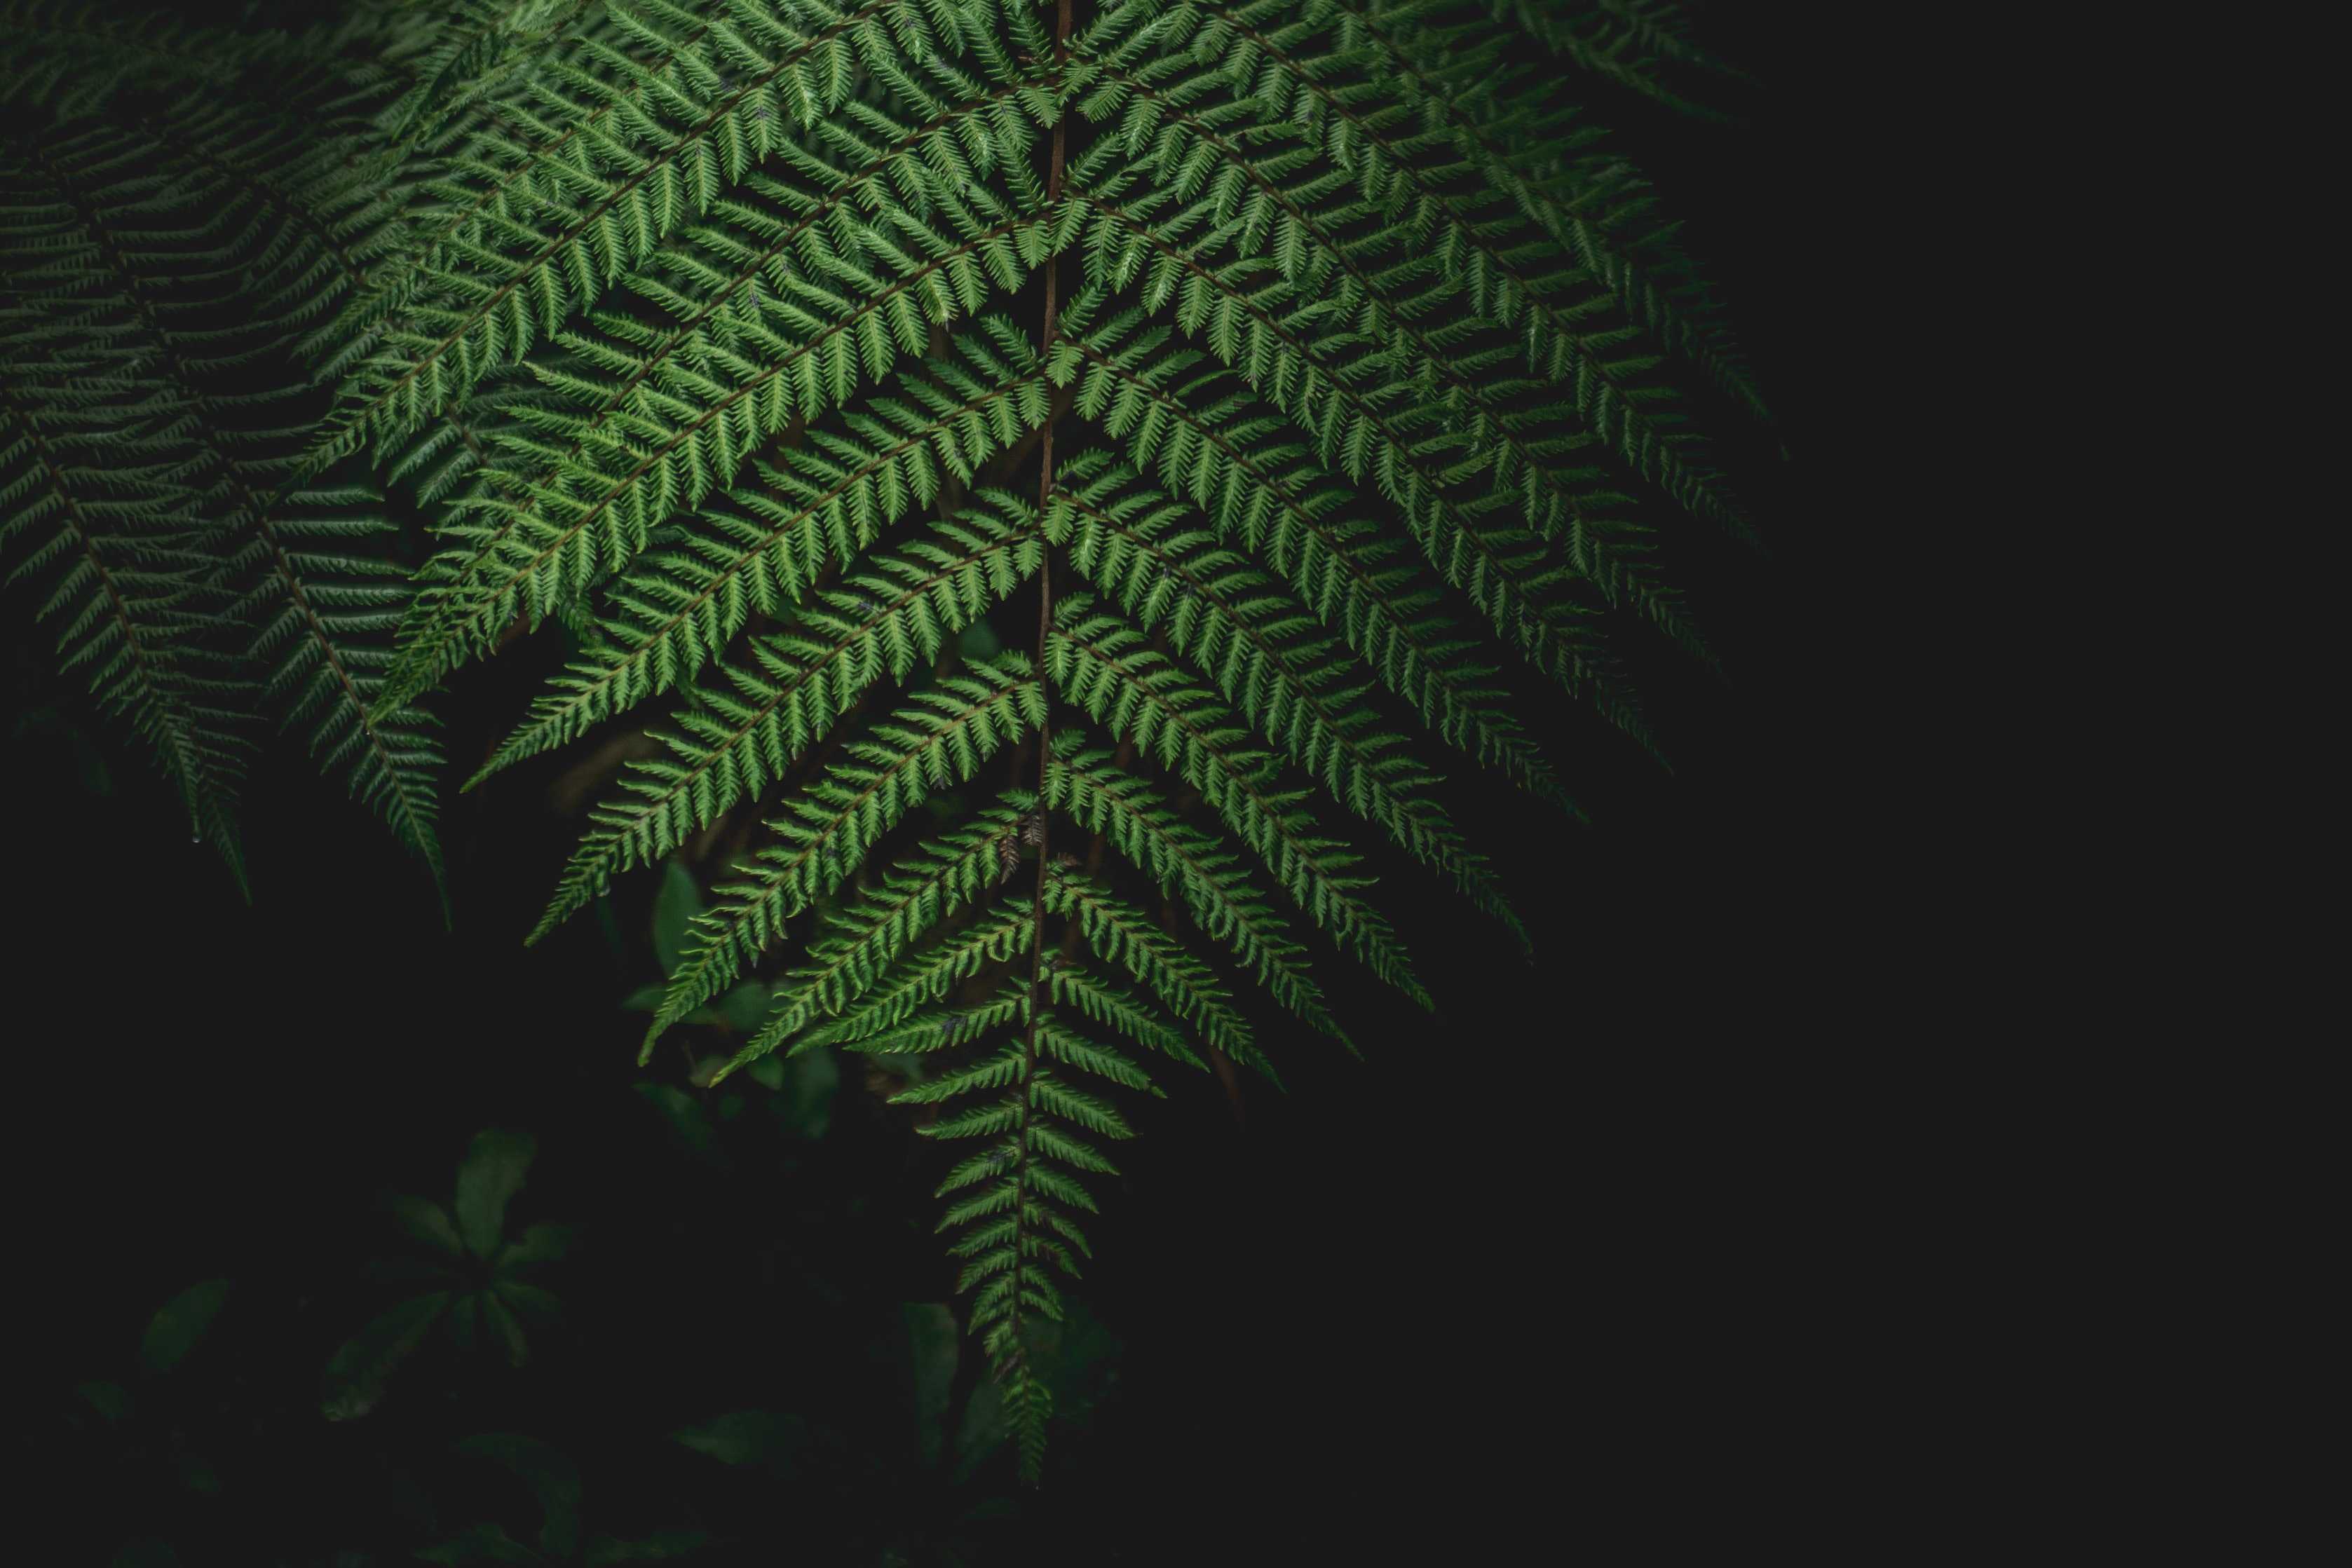
\includegraphics[height=1.0\paperheight, keepaspectratio]{racim-amr-9uKUR7TwNpU-unsplash.jpg}}
	\end{textblock*}

	% Cover author and title.
	\begin{textblock*}{0.8\coverwidth} (\frontcoveroffset, 50mm) % {block width} (coords)
		\fontsize{28}{33}\selectfont%
		John Dawson\par
		\vspace{12em}%
		\raggedleft%
		\fontsize{44}{52}\selectfont%
		\textbf{Forest Vines}\emph{ to}\par
		\textbf{Snow Tussocks}\par
		\vspace{0.5em}
		\fontsize{28}{33}\selectfont%
		The story of New Zealand plants
	\end{textblock*}

	% Spine title and author. Use a 1pt width and reduce the spine offset by about half the font size.
	\begin{textblock*}{1pt} (\spineoffset-7pt, 50mm)
		\centering%
		\begin{rotate}{-90}
			\fontsize{18}{18}\selectfont%
			\textbf{Forest Vines to Snow Tussocks\hspace{11em}John Dawson}
		\end{rotate}
	\end{textblock*}

	% Back cover.
	\begin{textblock*}{0.66\coverwidth} (\backcoveroffset, 40mm)
		\Large\centering%
		\setlength{\parskip}{1em}%
		Forest Vines to Snow Tussocks is the first general review of the distinctive features of New Zealand native plants since Cockayne's \emph{New Zealand Plants and their Story}, now long out of print.

		The plant communities, from dense lowland forest to alpine tundra, provide the book's framework, and within this many interesting and often puzzling aspects are considered: vines, epiphytes and parasites of the forest; the many peculiar shrubs with minute leaves and densely interlaced twigs; and the dense cushion plants, or `vegetable sheep', of the high mountains.

		Although more than 80 percent of New Zealand's native plants are found nowhere else our flora does not stand alone, so comparisons are made with the plants of other southern lands.

		In the last chapter an attempt is made to reconstruct the history of the New Zealand flora over geological time.

		\emph{Forest Vines to Snow Tussocks} fills an important gap in New Zealand's botanical literature — a fascinating and invaluable book for student and general reader alike.
		
		\vspace{5em}%
		{\small Cover photo by Racim Amr (https://unsplash.com/@therealracim)}
	\end{textblock*}

	% Load the ISBN graphic if defined.
	\ISBNgraphic{}

\end{document}
